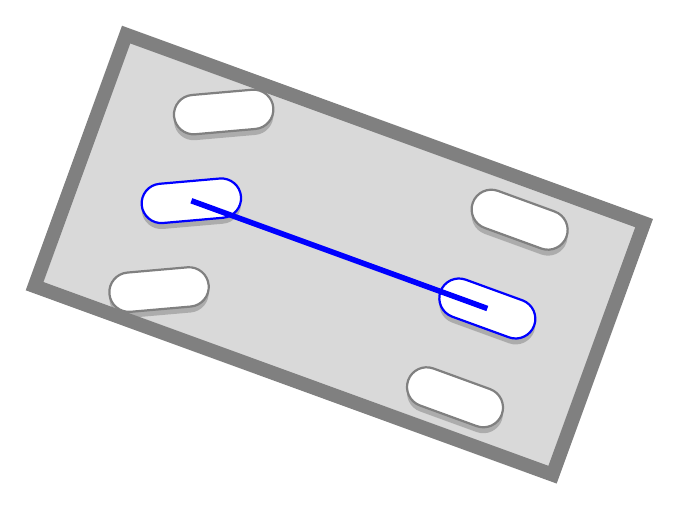
\begin{tikzpicture}
\usetikzlibrary{shapes.misc,shadows}
\usetikzlibrary{calc}
\usetikzlibrary{positioning,backgrounds}

\pgfmathsetmacro{\dist}{4}
\pgfmathsetmacro{\deltavar}{25}
\pgfmathsetmacro{\ax}{tan(90-\deltavar)*\dist*(-1)}
\pgfmathsetmacro{\vwh}{1.2}



\pgfmathsetmacro{\myrot}{70}
\pgfmathsetmacro{\myshift}{1}
%\pgfmathsetmacro{\myrot}{0}
%\pgfmathsetmacro{\myshift}{0}
\begin{scope}[shift={(0,\myshift)},rotate=\myrot]

% NODES

\draw  [line width = 5, gray, fill=gray!30!white] (-1.7,-1.5) rectangle (1.7,5.5);


\node(tire1)[draw=blue, thick, fill=white, 
			shape=rounded rectangle,  
			drop shadow={opacity=.5,shadow xshift=0pt},
			minimum width=1.5cm, 
			minimum height=0.5cm,
			rotate=90+\myrot]  at (0,0)   {};
			
\node(tire2)[draw=blue, thick, fill=white, 
			shape=rounded rectangle,  
			drop shadow={opacity=.5,shadow xshift=0pt},
			minimum width=1.5cm, 
			minimum height=0.5cm,
			rotate=\deltavar-90+\myrot]  at (0,\dist)   {};
			
\node(tireFL)[draw=gray, thick, fill=white, 
			shape=rounded rectangle,  
			drop shadow={opacity=.5,shadow xshift=0pt},
			minimum width=1.5cm, 
			minimum height=0.5cm,
			rotate=90+\myrot]  at (-\vwh,0)   {};
			
\node(tireBL)[draw=gray, thick, fill=white, 
			shape=rounded rectangle,  
			drop shadow={opacity=.5,shadow xshift=0pt},
			minimum width=1.5cm, 
			minimum height=0.5cm,
			rotate=\deltavar-90+\myrot]  at (-\vwh,\dist)   {};

\node(tireFR)[draw=gray, thick, fill=white, 
			shape=rounded rectangle,  
			drop shadow={opacity=.5,shadow xshift=0pt},
			minimum width=1.5cm, 
			minimum height=0.5cm,
			rotate=90+\myrot]  at (\vwh,0)   {};
			
\node(tireBR)[draw=gray, thick, fill=white, 
			shape=rounded rectangle,  
			drop shadow={opacity=.5,shadow xshift=0pt},
			minimum width=1.5cm, 
			minimum height=0.5cm,
			rotate=\deltavar-90+\myrot]  at (\vwh,\dist)   {};



\draw[line width=2, color=blue]  (tire1.center) -- (tire2.center); 

% angle delta top
%\draw[dashed] (0, \dist) -- (0,\dist+2);
%\draw[dashed] (0, \dist) -- ({-sin(\deltavar)*2},{\dist+2)});
%\draw[color=black] (0,\dist+1.5) arc (90:90+\deltavar:1.5);
%\draw (-0.2, \dist+1.1) node[black] {$\delta$};


\end{scope}

\end{tikzpicture}